% Author: Jan Schaumann <jschauma@netmeister.org>
% $Id: slides.tex,v 1.5 2006/04/10 14:22:04 jschauma Exp $
\special{! TeXDict begin /landplus90{true}store end }

\documentclass[xga]{xdvislides}
\usepackage[landscape]{geometry}
\usepackage{graphics}
\usepackage{graphicx}
\usepackage{colordvi}
\usepackage{multirow}
\usepackage[normalem]{ulem}

\begin{document}
\setfontphv

%%% Headers and footers
\lhead{\slidetitle}                               % default:\lhead{\slidetitle}
\chead{CS615 - Aspects of System Administration}% default:\chead{\relax}
\rhead{Slide \thepage}                       % default:\rhead{\sectiontitle}
\lfoot{\Gray{Popular Services -- HTTPS, Monitoring}}% default:\lfoot{\slideauthor}
\cfoot{\relax}                               % default:\cfoot{\relax}
\rfoot{\Gray{\today}}

\newcommand{\smallish}{\fontsize{16}{16}\selectfont}

\vspace*{\fill}
\begin{center}
	\Hugesize
		CS615 - Aspects of System Administration\\ [1em]
		Popular Services -- HTTPS, Monitoring\\ [1em]
	\hspace*{5mm}\blueline\\ [1em]
	\Normalsize
		Department of Computer Science\\
		Stevens Institute of Technology\\
		Jan Schaumann\\
		\verb+jschauma@stevens.edu+\\
		\verb+https://www.cs.stevens.edu/~jschauma/615/+
\end{center}
\vspace*{\fill}

\subsection{HTTP}
\begin{verbatim}
http://www.cs.stevens.edu/~jschauma/tmp/request.html
\end{verbatim}

\subsection{HTTP}
\small
\begin{verbatim}
IP 10.89.92.9.50777 > 155.246.89.84.80: Flags [P.], seq 1:639, ack 1, length 638
[...]
        0x0030:  8917 fc49 504f 5354 202f 7e6a 7363 6861  ...IPOST./~jscha
        0x0040:  756d 612f 6367 692d 6269 6e2f 706f 7374  uma/cgi-bin/post
        0x0050:  2e63 6769 2048 5454 502f 312e 310d 0a48  .cgi.HTTP/1.1..H
        0x0060:  6f73 743a 2077 7777 2e63 732e 7374 6576  ost:.www.cs.stev
        0x0070:  656e 732e 6564 750d 0a43 6f6e 6e65 6374  ens.edu..Connect
        0x0080:  696f 6e3a 206b 6565 702d 616c 6976 650d  ion:.keep-alive.
[...]
        0x0150:  2031 0d0a 5573 6572 2d41 6765 6e74 3a20  .1..User-Agent:.
        0x0160:  4d6f 7a69 6c6c 612f 352e 3020 284d 6163  Mozilla/5.0.(Mac
        0x0170:  696e 746f 7368 3b20 496e 7465 6c20 4d61  intosh;.Intel.Ma
        0x0180:  6320 4f53 2058 2031 305f 3130 5f35 2920  c.OS.X.10_10_5).
        0x0190:  4170 706c 6557 6562 4b69 742f 3533 372e  AppleWebKit/537.
        0x01a0:  3336 2028 4b48 544d 4c2c 206c 696b 6520  36.(KHTML,.like.
        0x01b0:  4765 636b 6f29 2043 6872 6f6d 652f 3439  Gecko).Chrome/49
        0x01c0:  2e30 2e32 3632 332e 3131 3020 5361 6661  .0.2623.110.Safa
        0x01d0:  7269 2f35 3337 2e33 360d 0a43 6f6e 7465  ri/537.36..Conte
        0x01e0:  6e74 2d54 7970 653a 2061 7070 6c69 6361  nt-Type:.applica
        0x01f0:  7469 6f6e 2f78 2d77 7777 2d66 6f72 6d2d  tion/x-www-form-
        0x0200:  7572 6c65 6e63 6f64 6564 0d0a 444e 543a  urlencoded..DNT:
        0x0210:  2031 0d0a 4163 6365 7074 2d45 6e63 6f64  .1..Accept-Encod
        0x0220:  696e 673a 2067 7a69 702c 2064 6566 6c61  ing:.gzip,.defla
        0x0230:  7465 0d0a 4163 6365 7074 2d4c 616e 6775  te..Accept-Langu
        0x0240:  6167 653a 2065 6e2d 5553 2c65 6e3b 713d  age:.en-US,en;q=
        0x0250:  302e 380d 0a43 6f6f 6b69 653a 205f 5f63  0.8..Cookie:.__c
        0x0260:  6664 7569 643d 6438 6530 3466 6365 3065  fduid=d8e04fce0e
        0x0270:  6136 6136 3133 6233 6466 3439 6130 3730  a6a613b3df49a070
        0x0280:  3631 3932 3532 6331 3436 3033 3931 3630  619252c146039160
        0x0290:  310d 0a0d 0a64 6174 613d 7468 6973 2b69  1....data=this+i
        0x02a0:  732b 612b 7365 6372 6574 2b6d 6573 7361  s+a+secret+messa
        0x02b0:  6765 ge
\end{verbatim}
\Normalsize


\subsection{HTTPS}
\begin{verbatim}
https://www.cs.stevens.edu/~jschauma/tmp/request.html
\end{verbatim}

\subsection{HTTPS}
\small
\begin{verbatim}
IP 155.246.89.84.443 > 10.89.92.9.50833: Flags [P.], seq 138:634, ack 1237, length 496
        0x0000:  4500 0224 de34 4000 3406 0af3 9bf6 5954  E..$.4@.4.....YT
        0x0010:  0a59 5c09 01bb c691 2042 e9c5 971f 45d4  .Y\......B....E.
        0x0020:  8018 0210 0f8a 0000 0101 080a 891a 57ec  ..............W.
        0x0030:  3d76 29d4 1703 0301 0515 a4d7 9c25 9a45  =v)..........%.E
        0x0040:  653d ee2c d8d7 d53e 045f a778 5cab e270  e=.,...>._.x\..p
        0x0050:  7d78 e20e c565 ca3e 41bb e3dc e428 8ae7  }x...e.>A....(..
        0x0060:  425b af7f a3cf ea8e 1179 0c2a 9385 0d76  B[.......y.*...v
        0x0070:  e328 f40b c972 e95f 67db 7f10 230f 4b54  .(...r._g...#.KT
        0x0080:  e675 5bdb 7cc7 b00a 49cd 645a 0e7c 4cf8  .u[.|...I.dZ.|L.
        0x0090:  7120 dc31 d1e5 b3f4 5b5c 6e57 e43c f6aa  q..1....[\nW.<..
        0x00a0:  7499 6046 dce6 0152 098e 3fca 66ac 5929  t.`F...R..?.f.Y)
        0x00b0:  5777 6c2f 2658 eca1 5fa6 3ef6 476f 42fe  Wwl/&X.._.>.GoB.
        0x00c0:  c2b6 4948 4194 f23a ced9 2a67 cf7d bbc3  ..IHA..:..*g.}..
        0x00d0:  2046 ad15 233c ffd2 3321 849b cf88 4233  .F..#<..3!....B3
        0x00e0:  515e be8f 03c0 786b f0e6 bec7 f961 7996  Q^....xk.....ay.
        0x00f0:  f352 6a1c 0968 726e 819a c927 2e69 358c  .Rj..hrn...'.i5.
        0x0100:  fb57 c9ae 7962 06d5 3529 210a 22d8 9eda  .W..yb..5)!."...
        0x0110:  9c30 e8a8 6ccf d30c 4bfc e689 7a8f 6ec4  .0..l...K...z.n.
        0x0120:  f232 9c14 6394 39f1 56e6 3e8a c910 e8b4  .2..c.9.V.>.....
        0x0130:  79c8 44ca dde0 8cc6 3a4a e4c4 ec15 1703  y.D.....:J......
        0x0140:  0300 2215 a4d7 9c25 9a45 66b1 c56f b2c4  .."....%.Ef..o..
        0x0150:  de96 6808 09b6 b553 9de1 cd6e 9adc cb99  ..h....S...n....
        0x0160:  9099 642e 1817 0303 0095 15a4 d79c 259a  ..d...........%.
        0x0170:  4567 617a 87ea e56d ce1f c2f0 6101 a7dd  Egaz...m....a...
        0x0180:  bfbe 756b cc50 26fb af35 1ffc e842 c1cc  ..uk.P&..5...B..
        0x0190:  5bae cc33 3110 ac66 bf43 7897 fad8 5e80  [..31..f.Cx...^.
        0x01a0:  509e 7305 e58b 1aaf 0e96 76b0 aa24 f900  P.s.......v..$..
        0x01b0:  290a 9260 6052 6ac0 6bd3 f8c6 f873 8bfb  )..``Rj.k....s..
        0x01c0:  af6f ee9c 0a35 7e9c ca18 7adc 9cd9 e2cc  .o...5~...z.....
        0x01d0:  8cec 4034 4970 bf94 4cce 0adb 3778 7648  ..@4Ip..L...7xvH
        0x01e0:  10c7 3505 09fd ff80 fe27 7b1d 34ac c066  ..5......'{.4..f
\end{verbatim}
\Normalsize

\subsection{HTTPS}
HTTPS stands for... \\

HTTP over SSL.

\subsection{HTTPS}
HTTPS stands for... \\

\sout{HTTP over SSL.} \\

HTTP over TLS.

\subsection{HTTPS}
HTTPS stands for... \\

\sout{HTTP over SSL.} \\

\sout{HTTP over TLS.} \\

Secure HTTP.

\subsection{HTTPS}
HTTPS stands for... \\

\sout{HTTP over SSL.} \\

\sout{HTTP over TLS.} \\

\sout{Secure HTTP.} \\

HTTP Secure.

\subsection{HTTPS}
HTTPS stands for... \\

\sout{HTTP over SSL.} \\

\sout{HTTP over TLS.} \\

\sout{Secure HTTP.} \\

HTTP Secure. \\

But it uses TLS.  And used to use SSL. Although
hopfully not any more.  Although probably still. \\

SSL is dead.  Don't use it.  Seriously, don't. \\

We should really only call it TLS.  HTTPT.

\subsection{TLS}
\begin{center}
	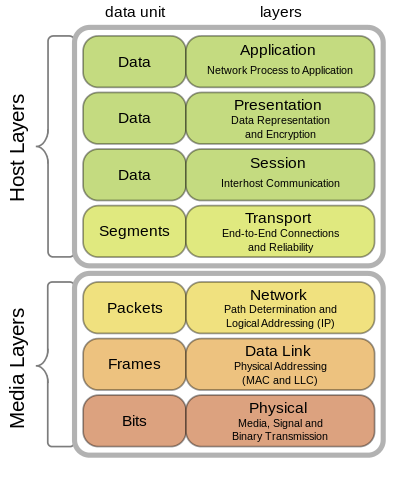
\includegraphics[scale=0.7]{pics/OSI_Model.eps}
\end{center}

\subsection{TLS}
Transport Layer Security
\begin{itemize}
	\item set of cryptographic protocols
	\item operates on layer 6 of OSI stack (Presentation Layer)
	\item independent of HTTP
	\item RFC5246 (TLS 1.2)
\end{itemize}
\addvspace{.5in}
Two distinct security mechanisms:
\begin{enumerate}
	\item encryption of data in transit
	\item authentication of parties
\end{enumerate}

\subsection{TLS}
Protocol:
\begin{itemize}
	\item Client Hello, present list of supported cipher suites
	\item Server Hello, chosen cipher suite
	\item Server Certificate
	\item (Server Key Exchange Message), (Client Certificate Request), (Client Certificate)
	\item Client Key Exchange Message
	\item (Certificate Verify)
	\item (Client Change Cipher Spec), (Server Change Cipher Spec)
\end{itemize}

\subsection{TLS}
\begin{center}
	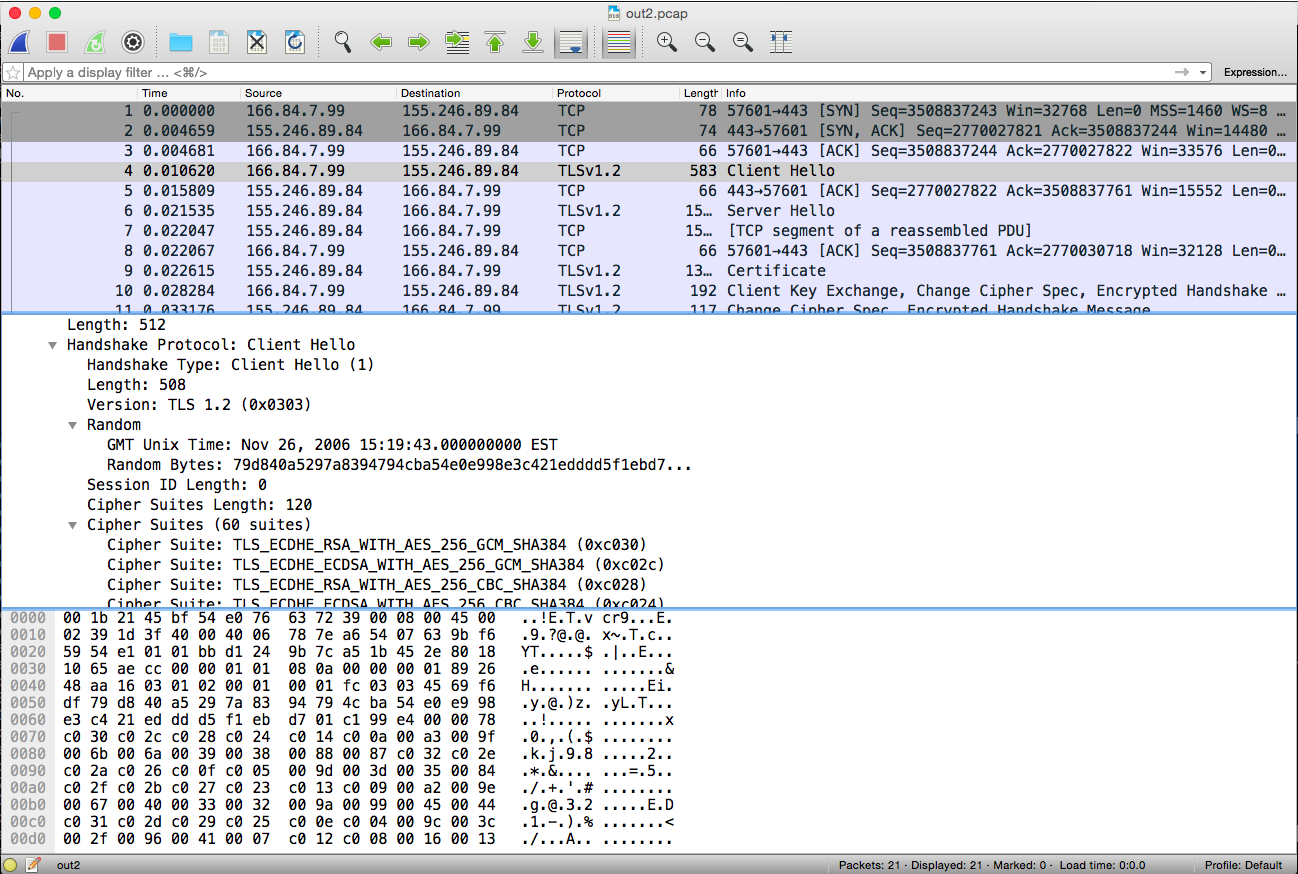
\includegraphics[scale=0.4]{pics/wireshark.eps}
\end{center}

\subsection{TLS}
\begin{verbatim}
$ openssl s_client -connect www.cs.stevens.edu:443
[...]
New, TLSv1/SSLv3, Cipher is DHE-RSA-AES256-SHA
Server public key is 2048 bit
Secure Renegotiation IS supported
Compression: NONE
Expansion: NONE
SSL-Session:
    Protocol  : TLSv1
    Cipher    : DHE-RSA-AES256-SHA
    Session-ID: 5F8A9B7A93EF87009EFCC17BBD68938C56EAACD9DF4C3643EF034D047C9F44C9
    Session-ID-ctx: 
    Master-Key: 20CBA1E477A8B573F29759045329EF7AA38C763C4C41606A46FBCC824C3F32F708789311E7B4275470E35CF09518FDCD
    Key-Arg   : None
    Start Time: 1460395966
    Timeout   : 300 (sec)
    Verify return code: 0 (ok)
\end{verbatim}

\subsection{TLS}
\begin{verbatim}
$ openssl s_client -connect www.cs.stevens.edu:443 | \
        openssl x509 -text -noout
[...]
        Signature Algorithm: sha1WithRSAEncryption
        Issuer: C=US, ST=Arizona, L=Scottsdale, O=GoDaddy.com, Inc., OU=http://certificates.godaddy.com/repository, CN=Go Daddy Secure Certification Authority/serialNumber=07969287
        Validity
            Not Before: Apr 22 13:14:11 2013 GMT
            Not After : Nov  8 15:26:38 2016 GMT
        Subject: OU=Domain Control Validated, CN=www.srcit.stevens.edu
        Subject Public Key Info:
            Public Key Algorithm: rsaEncryption
            RSA Public Key: (2048 bit)
[...]
            X509v3 Subject Alternative Name: 
                DNS:www.srcit.stevens.edu, DNS:srcit.stevens.edu, DNS:svn.srcit.stevens.edu,
                DNS:www.cs.stevens.edu, DNS:guinness.cs.stevens.edu, DNS:rcs.srcit.stevens.edu
\end{verbatim}

\subsection{TLS}
Setting up a Man in the Middle attack site: \\

1. start instance \\

2. {\tt openssl req -x509 -nodes -days 365 -sha256 \
        -newkey rsa:2048 -keyout mycert.pem -out mycert.pem}

3. {\tt sudo openssl s\_server -WWW -accept 443 -cert mycert.pem} \\

4. {\tt curl https://www.stevens.edu/sit/ > index.html} \\

4. go to {\tt https://<instance>/} \\

\subsection{TLS Authentication}
Use of X.509:
\begin{itemize}
	\item public key certificates
	\item certificate revocation lists (CRLs) / Online Certificate Status Protocol (OCSP)
	\item certificate path validation under a Public Key Infrastructure (PKI)
	\item certificate chains depend on trust anchors
\end{itemize}

\subsection{TLS}
\begin{center}
	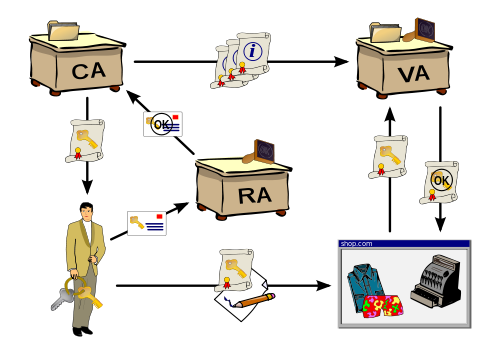
\includegraphics[scale=0.8]{pics/pki.eps} \\
CA = Certificate Authority;  RA = Registration Authority; \\
VA = Validation Authority
\end{center}

\subsection{TLS}
1. User / Company generates a {\em Certificate Signing Request} (CSR),
containing:

\begin{itemize}
	\item identifying information (distinguished name etc.)
	\item signature of data by private key
	\item chosen public key
\end{itemize}

\subsection{TLS}
1. User / Company generates a {\em Certificate Signing Request} (CSR) \\

2. CSR submitted to Certificate Authority (CA) \\

\subsection{TLS}
1. User / Company generates a {\em Certificate Signing Request} (CSR) \\

2. CSR submitted to Certificate Authority (CA) \\

3. CA verifies information \\

\subsection{TLS}
1. User / Company generates a {\em Certificate Signing Request} (CSR) \\

2. CSR submitted to Certificate Authority (CA) \\

3. CA verifies information \\

4. CA returns certificate signed with its private key \\

\subsection{TLS}
1. User / Company generates a {\em Certificate Signing Request} (CSR) \\

2. CSR submitted to Certificate Authority (CA) \\

3. CA verifies information \\

4. CA returns certificate signed with its private key \\

5. clients can verify signatures against trusted {\em root CAs} \\

\subsection{TLS Pitfalls}
\begin{center}
	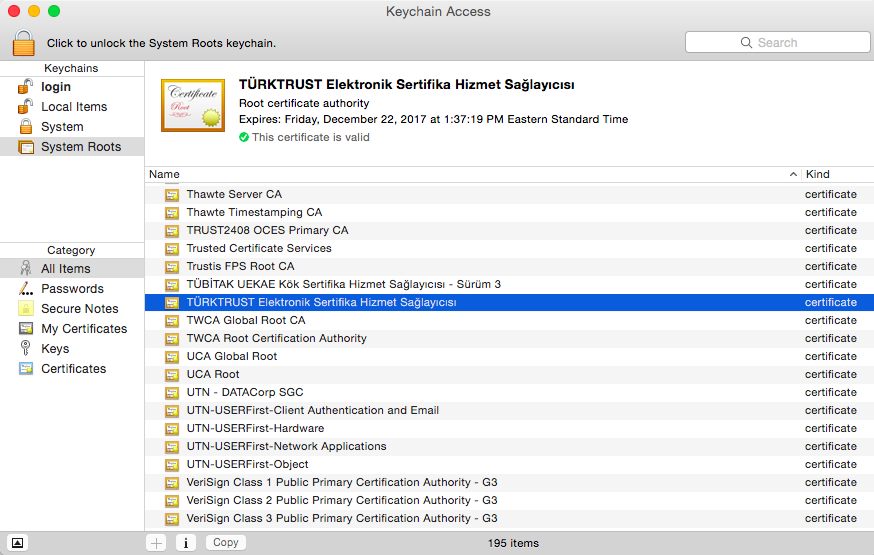
\includegraphics[scale=0.6]{pics/roots.eps} \\
	195 root CAs on this laptop...
\end{center}

\subsection{TLS Pitfalls}
Lack of universal HTTPS exposes users to significant
risks; many sites don't get the importance of
authentication for non-sensitive content. \\

In order to serve content, you need to have the
private key $ => $ privkey available at perimeter and
exposed, high-risk systems. \\

Rotation/renewal of keys requires routine processes,
which further expose the private key. \\

Control of a CA or a CA's key grants you near
universal powers. \\


\subsection{TLS Pitfalls}
Complex protocols, buggy implementations, intentional
weaknesses and backwards compatibility are just the
high level points.

\begin{itemize}
	\item SSLv2 obsoleted in 1996; 2016: DROWN attack
	\item SSLv3 obsoleted in 1999; 2014: POODLE attack
	\item BEAST, CRIME, BREACH, HEARTBLEED, GotoFail...
	\item obsolete and broken algorithms widely used (RC4, MD5, SHA1, ...)
\end{itemize}

\subsection{TLS}
Additional related topics:
\begin{itemize}
	\item HSTS and TLS stripping attacks
	\item HPKP and Trust On First Use (TOFU)
	\item Content Security Policy (CSP)
	\item ``Secure'' cookies vs. HttpOnly cookies
	\item attacks on domain name registrars
\end{itemize}
\addvspace{.5in}
Security is difficult.  More on that in a future
lecture.

\newpage
\vspace*{\fill}
\begin{center}
	\Hugesize
		Hooray!\\ [1em]
	\hspace*{5mm}
	\blueline\\
	\hspace*{5mm}\\
		5 minute break
\end{center}
\vspace*{\fill}

\subsection{Problem Report}
\vspace*{\fill}
\Huge
\begin{center}
``Something's wrong.''
\end{center}
\Normalsize
\vspace*{\fill}

\subsection{Now what?}
\begin{center}
	
\includegraphics[scale=0.55]{pics/monkey.eps}
\end{center}

\subsection{Problem Report}
\vspace*{\fill}
\Huge
\begin{center}
``The system feels slow.'' \\
\addvspace{.5in}
``I can't log in.'' \\
\addvspace{.5in}
``My mail was not delivered.'' \\
\addvspace{.5in}
``The site is down.''
\end{center}
\Normalsize
\vspace*{\fill}

\subsection{Now what?}
\begin{center}
	
\includegraphics[scale=0.55]{pics/monkey.eps}
\end{center}

\subsection{To the logs!}
\begin{center}
	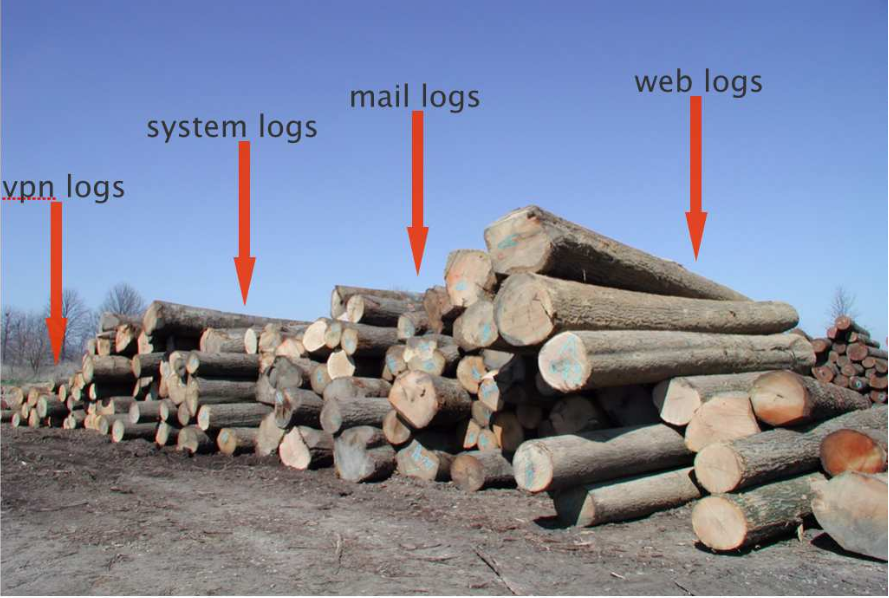
\includegraphics[scale=0.55]{pics/logs.eps}
\end{center}

\subsection{Answers}
``The system feels slow.''
\begin{verbatim}
up 1318 days, 13:46, 1 user, load averages: 993.81, 272.91, 1012.18}
\end{verbatim}

\addvspace{.3in}
``I can't log in.''
\begin{verbatim}
Apr 6 09:25:56 <auth.info>hostname sshd[1624]: Failed password for jdoe from
115.239.231.100 port 1047 ssh2}
\end{verbatim}

\addvspace{.3in}
``My mail was not delivered.''
\begin{verbatim}
Apr 11 16:15:40 panix postfix/smtpd[7566]: connect from unknown[122.3.68.122]
Apr 11 16:15:41 panix postfix/smtpd[7566]: NOQUEUE: reject_warning: RCPT from
unknown[122.3.68.122]: 450 4.7.1 Client host rejected: cannot find your hostname,
[122.3.68.122]; from=<McneilRomany28@pldt.net> to=<jschauma@stevens.edu>
proto=ESMTP helo=<122.3.68.122.pldt.net>
\end{verbatim}

\subsection{Answers}
``The site is down.'' \\

\begin{verbatim}
94.242.252.41 - "" [11/Apr/2016:19:18:47 -0400] "GET /secret/ HTTP/1.1"
403 524 "-" "Mozilla/5.0 (Macintosh; Intel Mac OS X 10.9; rv:28.0)
Gecko/20100101 Firefox/28.0"
\end{verbatim}

\subsection{Answers}
``The site is down.'' \\

\begin{verbatim}
94.242.252.41 - "" [11/Apr/2016:19:18:47 -0400] "GET /secret/ HTTP/1.1"
403 524 "-" "Mozilla/5.0 (Macintosh; Intel Mac OS X 10.9; rv:28.0)
Gecko/20100101 Firefox/28.0"
\end{verbatim}

\addvspace{.2in}
\begin{center}
	
\includegraphics[scale=0.25]{pics/monkey.eps}
\end{center}

\subsection{Events}
\vspace*{\fill}
\Huge
\begin{center}
``Something's wrong.'' is just an {\em unexpected} or
{\em undesirable} event.
\end{center}
\Normalsize
\vspace*{\fill}

\subsection{Events}
\vspace*{\fill}
\Huge
\begin{center}
``Something's wrong.'' is just an {\em unexpected} or
{\em undesirable} event. \\
\vspace{.4in}
{\em Events} happen all the time.
\end{center}
\Normalsize
\vspace*{\fill}

\subsection{Events}
\vspace*{\fill}
\Huge
\begin{center}
``Something's wrong.'' is just an {\em unexpected} or
{\em undesirable} event. \\
\vspace{.4in}
{\em Events} happen all the time. \\
\vspace{.4in}
Being able to identify {\em relevant} events allows
you to diagnose, predict and even prevent {\em
undesirable} events.
\end{center}
\Normalsize
\vspace*{\fill}

\subsection{Events}
\vspace*{\fill}
\Huge
\begin{center}
In order to be able to identify an event as {\em
unexpected}, you have to have {\em expected} events.
\end{center}
\Normalsize
\vspace*{\fill}

\subsection{Expected Events}
\vspace*{\fill}
\Huge
\begin{center}
Know your applications.
\end{center}
\Normalsize
\vspace*{\fill}

\subsection{Expected Events}
\vspace*{\fill}
\Huge
\begin{center}
Know your applications. \\
\vspace{.4in}
Know your users.
\end{center}
\Normalsize
\vspace*{\fill}

\subsection{Expected Events}
\vspace*{\fill}
\Huge
\begin{center}
Know your applications. \\
\vspace{.4in}
Know your users. \\
\vspace{.4in}
Know your traffic patterns.
\end{center}
\Normalsize
\vspace*{\fill}

\subsection{Expected Events}
\vspace*{\fill}
\Huge
\begin{center}
Know your applications. \\
\vspace{.4in}
Know your users. \\
\vspace{.4in}
Know your traffic patterns. \\
\vspace{.4in}
{\em Know your systems.}
\end{center}
\Normalsize
\vspace*{\fill}

\subsection{Events and Metrics}
\vspace*{\fill}
\begin{verbatim}
$ dict event
  event
      n 1: something that happens at a given place and time
      2: a special set of circumstances; "in that event, the first
         possibility is excluded"; "it may rain in which case the
         picnic will be canceled" [syn: {event}, {case}]


$ dict metric
  metric
      3: a system of related measures that facilitates the
         quantification of some particular characteristic [syn:
         {system of measurement}, {metric}]

\end{verbatim}
\vspace*{\fill}

\subsection{Events and Metrics}
\begin{center}
	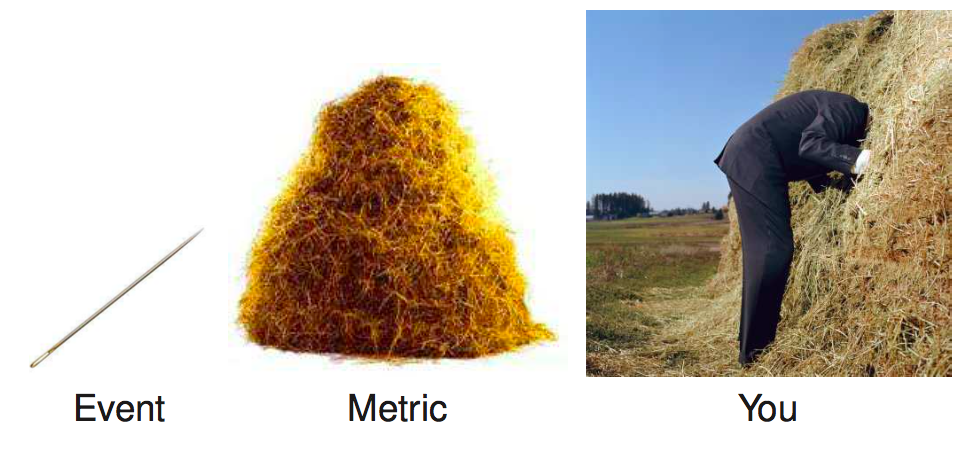
\includegraphics[scale=0.75]{pics/events-metrics.eps}
\end{center}

\subsection{Events and Metrics}
Events
\begin{itemize}
	\item may occur rarely / frequently / constantly
	\item can be collected in logs
	\item may be comprised of other events
	\item may be: ’something happened’
	\item may be: ’nothing (new) happened’
\end{itemize}
\addvspace{.5in}

Metrics:
\begin{itemize}
	\item correlation of related events
	\item may help identify outliers
	\item may trigger events
	\item may help make (automated or interactive) decisions
\end{itemize}


\subsection{Collecting Data}
{\em Counters}: easy, numeric data tracking individual events. Example: HTTP status codes

\addvspace{.5in}
{\em Timers}: easy, numeric data tracking event duration. Example: Time to send all
data for a successful HTTP request.

\addvspace{.5in}
{\em Thresholds}: easy, numeric trigger for events; may itself trigger events or metrics.
Example: more than N HTTP hits in X seconds yield 404.

\subsection{Counting counters, timing timers...}
SNMP
\vspace{.5in}
\begin{center}
	\Huge
	A complete network management system to monitor network-attached devices.
\end{center}
\Normalsize

\subsection{SNMP}
Base concepts:
\begin{itemize}
	\item managed devices run an {\em snmp agent} or d\ae mon
	\item information about the device is exposed in {\em management information bases}
	\item parts of a system are made available in {\em read-only} mode
	\item parts of a system may be made available in {\em write} mode
	\item certain conditions may trigger actions or {\em traps}
	\item normally uses UDP 161 for the {\em agent} and 162 for the {\em manager}
\end{itemize}

\subsection{SNMP}
Management Information Bases (MIBs):
\begin{itemize}
	\item hierarchical namespace
	\item contains {\em Object Identifiers} (OIDs)
	\item written in {\em Abstract Syntax Notation One} (ASN.1)
	\item often vendor defined
\end{itemize}

\subsection{SNMP Versions}
SNMPv1:
\begin{itemize}
	\item de-facto standard
	\item poor security (``community strings'' act as passwords)
\end{itemize}
\vspace{.2in}
SNMPv2:
\begin{itemize}
	\item improvements in the area of performance (\verb+GETBULK+ instead of \verb+GETNEXT+) and security
	\item comes in the flavors {\em SNMPv2c}, {\em SNMPv1.5} and {\em SNMPv2u}
\end{itemize}
\vspace{.2in}
SNMPv3:
\begin{itemize}
	\item official standard
	\item adds authentication, privacy and access control
\end{itemize}

\subsection{SNMP: An example}
\smallish
\begin{verbatim}
$ snmpwalk -c public -v 1 bluemoon.cs.stevens-tech.edu
iso.3.6.1.2.1.1.1.0 = STRING: "HP ETHERNET MULTI-ENVIRONMENT,ROM none,JETDIRECT,JD147,EEPROM
JDI2300 0013,CIDATE 07/13/2013"
iso.3.6.1.2.1.1.2.0 = OID: iso.3.6.1.4.1.11.2.3.9.1
iso.3.6.1.2.1.1.3.0 = Timeticks: (293219400) 33 days, 22:29:54.00
[...]
iso.3.6.1.2.1.25.3.2.1.3.1 = STRING: "HP Color LaserJet CP5520 Series"
iso.3.6.1.2.1.25.3.2.1.3.2 = STRING: "SanDisk SDSA5AK-008G-1006"
[...]
iso.3.6.1.2.1.43.16.5.1.2.1.1 = STRING: "Sleep mode on"
\end{verbatim}

\subsection{SNMP: An example}
\smallish
\begin{verbatim}
$ snmpwalk -c public -v 1 gw.cc.stevens-tech.edu
SNMPv2-MIB::sysDescr.0 = STRING: Cisco IOS Software, s72033_rp Software
(s72033_rp-ADVIPSERVICESK9_WAN-M), Version 12.2(33)SXH, RELEASE SOFTWARE (fc5)
DISMAN-EVENT-MIB::sysUpTimeInstance = Timeticks: (3112108803) 360 days, 4:44:48.03
SNMPv2-MIB::sysContact.0 = STRING: chose@stevens.edu x5457
SNMPv2-MIB::sysName.0 = STRING: gw.cc.stevens-tech.edu
SNMPv2-MIB::sysLocation.0 = STRING: campus:sl:0:machineroom
SNMPv2-MIB::sysORLastChange.0 = Timeticks: (0) 0:00:00.00
[...]
IF-MIB::ifPhysAddress.1 = STRING: 0:17:95:68:d2:dc
IF-MIB::ifPhysAddress.2 = STRING: 0:18:74:1c:e3:80
[...]
IF-MIB::ifAdminStatus.1 = INTEGER: up(1)
IF-MIB::ifAdminStatus.2 = INTEGER: down(2)
[...]
IF-MIB::ifInOctets.1 = Counter32: 147341347
IF-MIB::ifInOctets.2 = Counter32: 487894092
[...]
IF-MIB::ifOutOctets.1 = Counter32: 956876160
IF-MIB::ifOutOctets.2 = Counter32: 1532452749
[...]
RFC1213-MIB::ipRouteDest.66.193.255.0 = IpAddress: 66.193.255.0
RFC1213-MIB::ipRouteDest.66.194.0.0 = IpAddress: 66.194.0.0
[...]
\end{verbatim}
\Normalsize

\subsection{SNMP: An example}
\smallish
\begin{verbatim}
$ snmpwalk -Os -c public -v 1 localhost
iso.3.6.1.2.1.1.1.0 = STRING: "Linux avatar 3.2.0-51-generic #77-Ubuntu SMP Wed Jul 24 20:18:19
UTC 2013 x86_64"
iso.3.6.1.2.1.1.2.0 = OID: iso.3.6.1.4.1.8072.3.2.10
iso.3.6.1.2.1.1.3.0 = Timeticks: (31099465) 3 days, 14:23:14.65
[...]
iso.3.6.1.2.1.1.5.0 = STRING: "avatar"
iso.3.6.1.2.1.25.1.4.0 = STRING: "root=/dev/xvda2 ro
root=/dev/xvda2 ro ip=:127.0.255.255::::eth0:dhcp"
\end{verbatim}
\Normalsize

\subsection{Know Your Systems}
Profile your application:
\begin{itemize}
	\item execution time (for example: {\tt time(1)})
	\item data sources and destination affect execution
	\item {\tt strace(1)} and friends for more detailed analysis
\end{itemize}

\addvspace{.5in}
Understand your system performance:
\begin{itemize}
	\item CPU load, memory (for example: {\tt top(1)}, {\tt vmstat(1)})
	\item disk I/O (for example: {\tt iostat(1)})
	\item user activity (for example: {\tt ac(1)}, {\tt lsof(8)}, {\tt sa(8)})
\end{itemize}

\subsection{Know Your Systems}
Network statistics:
\begin{itemize}
	\item ports and applications (for example: {\tt lsof(8)}, {\tt netstat(8)})
	\item packets in and out
	\item connection origin
	\item {\em NetFlow} etc.
\end{itemize}

\subsection{Context}
{\em Context} lets you find {\em relevant} events in
your haystack of metrics.

\begin{center}
	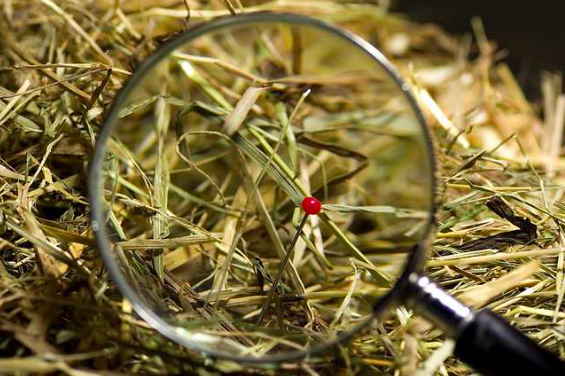
\includegraphics[scale=0.75]{pics/glass-needle.eps}
\end{center}

\subsection{No context.}
CPU load - 12 hours
\begin{center}
	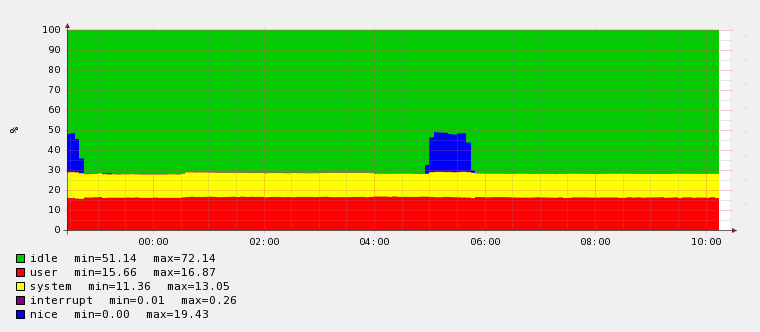
\includegraphics[scale=0.9]{pics/cpu-12h.eps}
\end{center}

\subsection{No context.}
Disk I/O - 12 hours
\begin{center}
	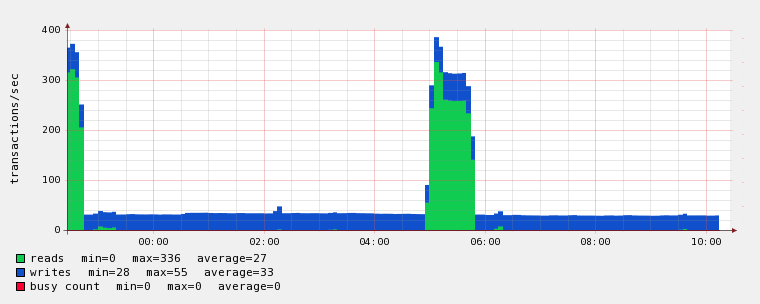
\includegraphics[scale=0.9]{pics/disk-io-12h.eps}
\end{center}

\subsection{No context.}
Load Average - 12 hours
\begin{center}
	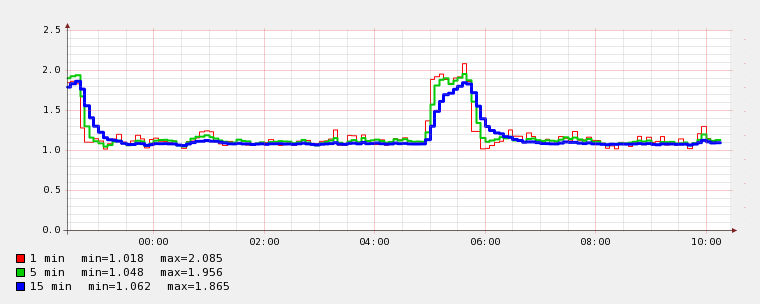
\includegraphics[scale=0.9]{pics/load-average-12h.eps}
\end{center}

\subsection{No context.}
Memory - 12 hours
\begin{center}
	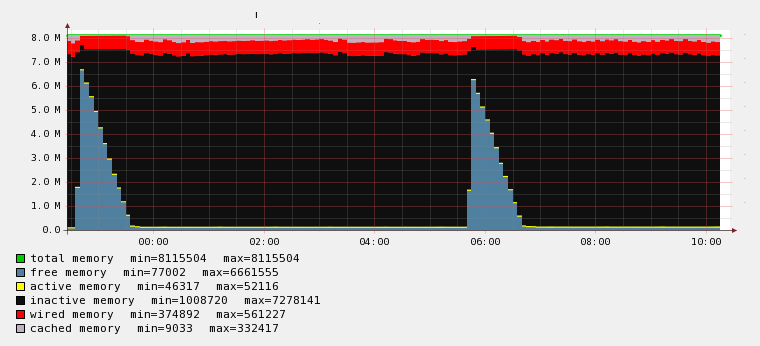
\includegraphics[scale=0.9]{pics/memory-12h.eps}
\end{center}

\subsection{Some context.}
12 hours
\begin{center}
	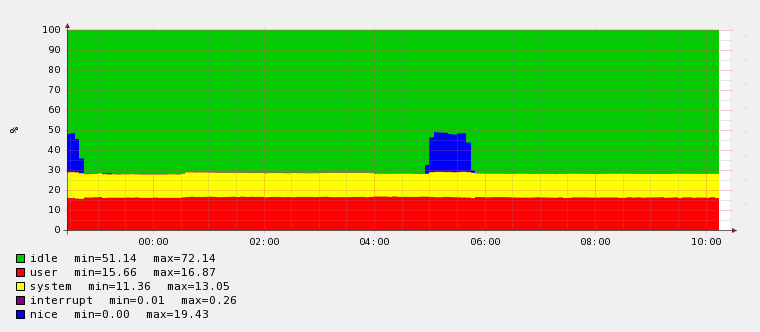
\includegraphics[scale=0.36]{pics/cpu-12h.eps}
	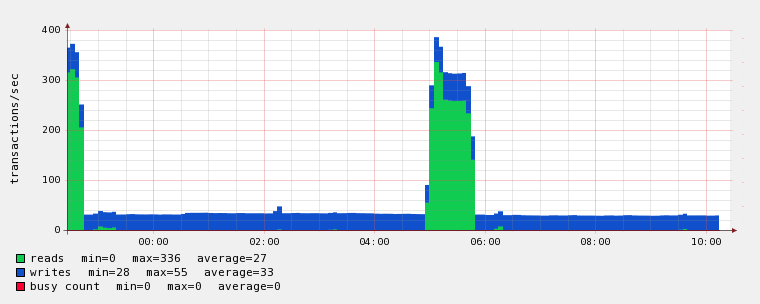
\includegraphics[scale=0.36]{pics/disk-io-12h.eps} \\
	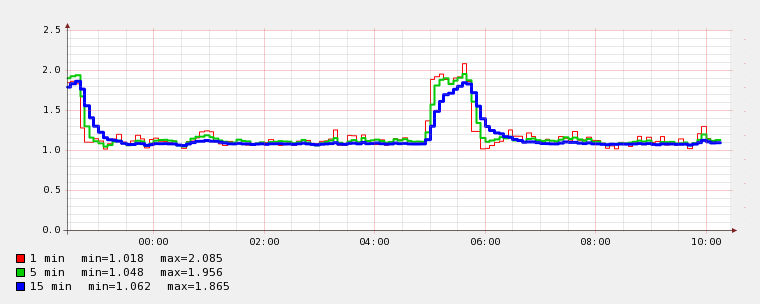
\includegraphics[scale=0.36]{pics/load-average-12h.eps}
	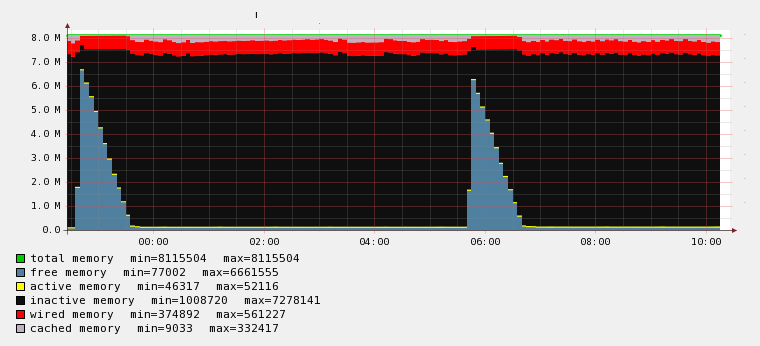
\includegraphics[scale=0.36]{pics/memory-12h.eps} \\
\end{center}

\subsection{With context.}
7 days
\begin{center}
	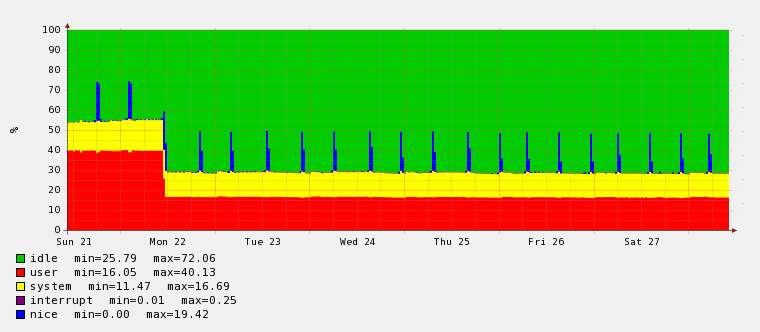
\includegraphics[scale=0.36]{pics/cpu-7day.eps}
	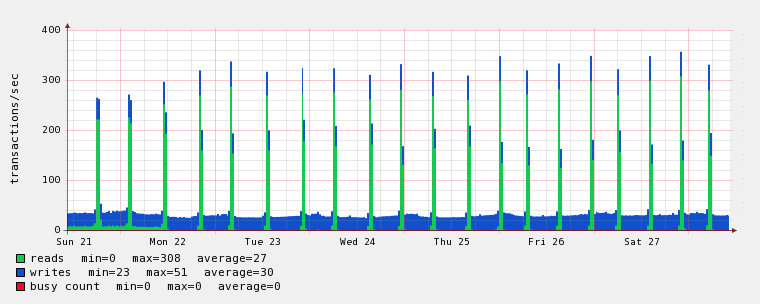
\includegraphics[scale=0.36]{pics/disk-io-7day.eps} \\
	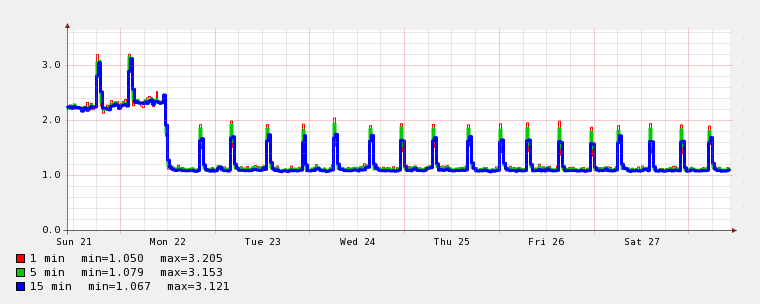
\includegraphics[scale=0.36]{pics/load-average-7day.eps}
	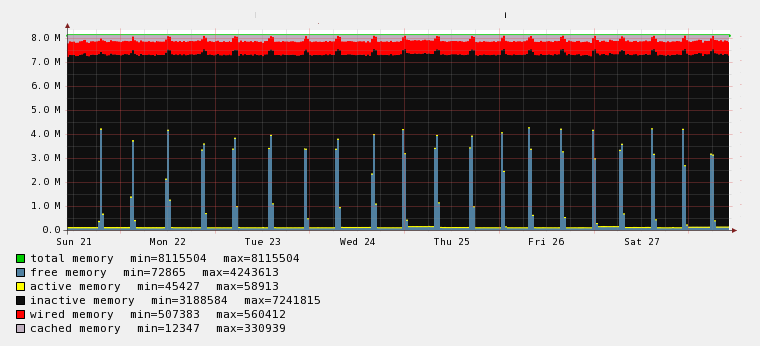
\includegraphics[scale=0.36]{pics/memory-7day.eps} \\
\end{center}

\subsection{Know your systems.}
CPU load - 30 days
\begin{center}
	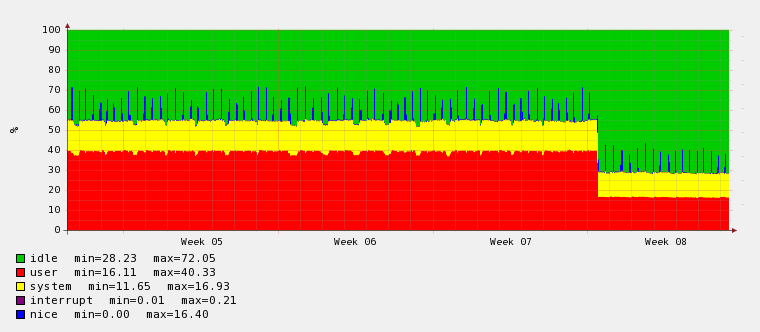
\includegraphics[scale=0.9]{pics/cpu-30day.eps}
\end{center}

\subsection{Know your systems.}
30 days
\begin{center}
	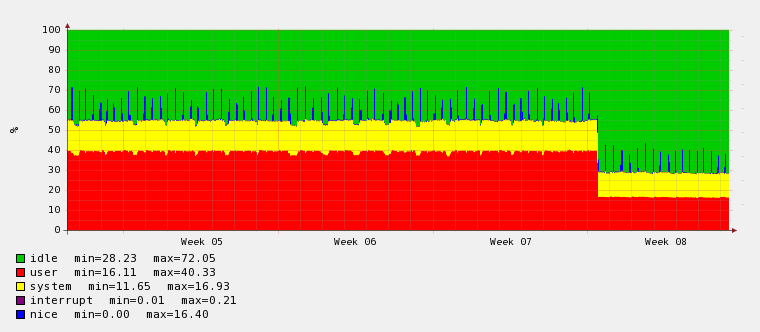
\includegraphics[scale=0.36]{pics/cpu-30day.eps}
	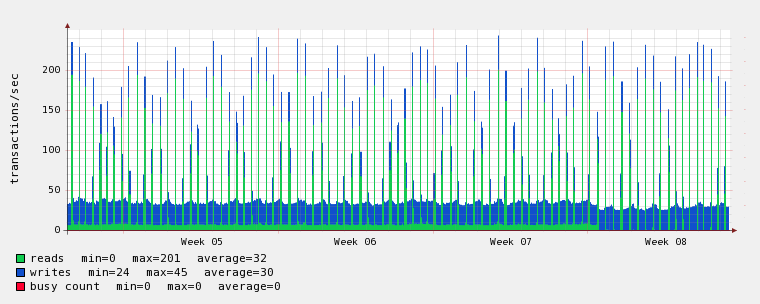
\includegraphics[scale=0.36]{pics/disk-io-30day.eps} \\
	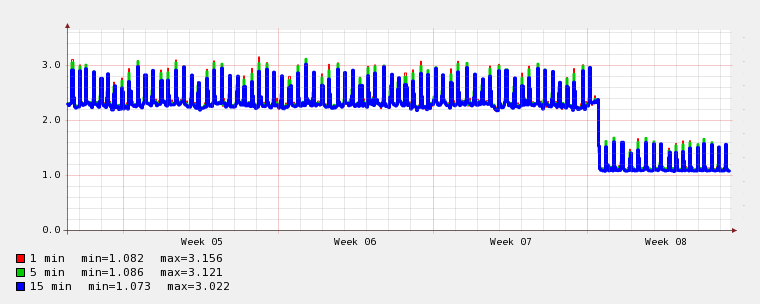
\includegraphics[scale=0.36]{pics/load-average-30day.eps}
	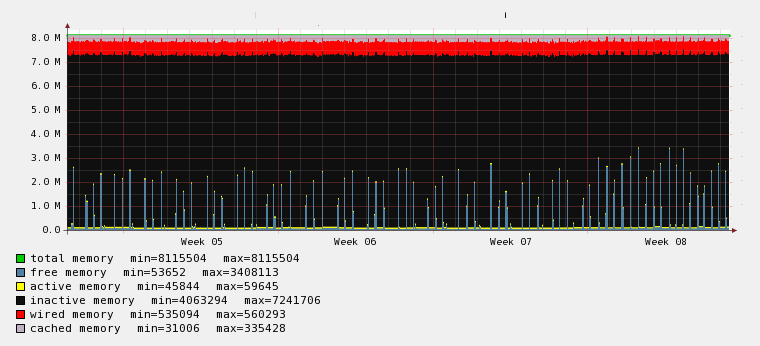
\includegraphics[scale=0.36]{pics/memory-30day.eps} \\
\end{center}

\subsection{Turn {\em events} into {\em metrics.}}
\begin{itemize}
	\item Log it!
\end{itemize}

\addvspace{.5in}
\begin{itemize}
	\item Export counters/timers from within your application.
	\item Process logs and produce counters/timers:
\begin{verbatim}
awk ’{print $9}’ /var/log/httpd/access.log | sort | uniq -c
\end{verbatim}
\end{itemize}

\addvspace{.5in}
\begin{itemize}
	\item Graph it. \\
	{\tt http://shouldigraphit.com/}
\end{itemize}

\subsection{Monitoring/graphing}
SNMP based:
\begin{itemize}
	\item Cacti: \verb+http://www.cacti.net/+
	\item MRTG: \verb+http://oss.oetiker.ch/mrtg/+
	\item Observium: \verb+http://demo.observium.org/+
	\item ...
\end{itemize}
\vspace{.2in}
Other / complementary:
\begin{itemize}
	\item Ganglia: \verb+http://monitor.millennium.berkeley.edu/+
	\item Munin: \verb+http://munin.ping.uio.no/+
	\item Nagios: \verb+http://nagioscore.demos.nagios.com/+
	\item Graphite: \verb+http://graphite.wikidot.com/+
\end{itemize}
\vspace{.5in}
%More on monitoring and performance in a future lecture (if time permits).

\subsection{To the cloud!}
There’s a service for that. In the cloud. \\

Consider:
\begin{itemize}
	\item support / convenience vs. do-it-yourself integration
	\item with your other services confidentiality
	\item data lock-in (esp. when trending data over years)
\end{itemize}

\subsection{Monitoring Pitfalls}
\vspace*{\fill}
\Huge
\begin{center}
Increasing the size of your haystack does not always
help in finding the needle.
\end{center}
\Normalsize
\vspace*{\fill}

\subsection{Monitoring Pitfalls}
\vspace*{\fill}
\Huge
\begin{center}
Increasing the size of your haystack does not always
help in finding the needle. \\
\vspace{.4in}
Email is not a scalable network monitoring solution.
\end{center}
\Normalsize
\vspace*{\fill}

\subsection{Monitoring Pitfalls}
\vspace*{\fill}
\Huge
\begin{center}
Increasing the size of your haystack does not always
help in finding the needle. \\
\vspace{.4in}
Email is not a scalable network monitoring solution. \\
\vspace{.4in}
Absence of a signal can itself be a signal.
\end{center}
\Normalsize
\vspace*{\fill}

\subsection{Monitoring Pitfalls}
\vspace*{\fill}
\Huge
\begin{center}
Increasing the size of your haystack does not always
help in finding the needle. \\
\vspace{.4in}
Email is not a scalable network monitoring solution. \\
\vspace{.4in}
Absence of a signal can itself be a signal. \\
\vspace{.4in}
This list is incomplete.
\end{center}
\Normalsize
\vspace*{\fill}

\subsection{Reading}
HTTPS / TLS:
\begin{itemize}
	\item {\tt https://en.wikipedia.org/wiki/HTTPS}
	\item RFC5246 (TLS 1.2) and RFC6176 (prohibiting SSL)
	\item {\tt https://bugzilla.mozilla.org/show\_bug.cgi?id=647959}
	\item {\tt https://cabforum.org}
\end{itemize}

\subsection{Reading}
SNMP:
\begin{itemize}
	\item \verb+http://is.gd/1LwOSD+
	\item RFCs 1157, 3411, 3418 and others
	\item \verb+snmpcmd(1)+
\end{itemize}

Monitoring:
\begin{itemize}
	\item {\tt https://www.slac.stanford.edu/xorg/nmtf/nmtf-tools.html}
	\item {\tt http://www.datadoghq.com/}
	\item {\tt https://www.newrelic.com/}
	\item {\tt http://logstash.net/}
	\item {\tt http://www.splunk.com/}
\end{itemize}

\end{document}
